\documentclass[12pt]{article}
\parindent=0.25in

\setlength{\oddsidemargin}{0pt}
\setlength{\textwidth}{440pt}
\setlength{\topmargin}{0in}
\usepackage{amssymb}
\usepackage{amsfonts}
\usepackage{amsmath}
\usepackage{cancel}
\usepackage{latexsym}
\usepackage[center]{subfigure}
\usepackage{epsfig}
\usepackage{3952}
\usepackage{3952-thm}
\usepackage{pstricks,pst-node,pst-tree}
\usepackage{soul, xcolor}
\usepackage{bbold}
\usepackage[shortlabels]{enumitem}
\usepackage[backref, colorlinks,citecolor=blue,bookmarks=true]{hyperref}  

\pagestyle{headings}    % Go for customized headings

\newcommand{\handout}[5]{
   \noindent
   \begin{center}
   \framebox{
      \vbox{
    \parbox[t]{4in} {\bf #1 } \vspace{3mm}  {\hfill \bf #2 }
       \vspace{2mm}
       \hbox to 6.00in { {\Large \hfill #5  \hfill} }
       \vspace{1mm}
       \hbox to 6.00in { {\it #3 \hfill #4} }
      }
   }
   \end{center}
   \vspace*{1mm}
}

\hypersetup{linkcolor=magenta}

\begin{document}

\handout{MATH 3952 (Undergraduate Seminar): Quantum Information Theory}{Spring 2024}
{Organizer: Patrick Lei; Presenter: Tasmim Rahman}
{Scribe: Mark Chen}{Lecture 6, Talk 2: March 4, 2024}

\thispagestyle{plain}
% \setcounter{section}{-1}
\section*{Chapter 6: Bell's Theorem (Ctd.)}
\section{Tsirelson's Inequality}
We have seen that $2\sqrt{2}$ is a quantum correlation value that beats the $2$ bound set up in the classical case. \textbf{Tsirelson's Inequality} establishes it also as the upper bound for quantum correlation.

\begin{proposition}
$\lr{S} = \Bra{\psi} S \Ket{\psi} \leq$ the largest eigenvalue of $S$.
\end{proposition}

\noindent So, the Goal now becomes to find the largest eigenvalue of a unitary $S$.

\begin{definition}[Matrix Norm of Hermitian Matrix]
Let $M, N$ be Hermitian matrix, then, we denote the \textbf{largest eigenvalue of them}, i.e. the \textbf{matrix norm} as $$
||M||\text{ and } ||N||\text{, respectively.}
$$
\end{definition}

\begin{definition}
The matrix norm as defined above have the following properties, again, given $M,N$ as Hermitian matrices:
\begin{itemize}
    \item $\|M\otimes N\| = \|M\| \|N\|$.
    \item $\|M N\| \leq \|M\| \|N\|$.
    \item $\|M + N\| \leq \|M\| + \|N\|$.
\end{itemize}
\end{definition}

\begin{remark}
Notice that, given $$
S = A_1B_1 - A_1B_2 + A_2B_1 + A_2B_2,
$$ it is easy to find that $$
\|S\| = \|A_1B_1 - A_1B_2 + A_2B_1 + A_2B_2\| \leq \|A_1B_1\| + \|A_1B_2\| + \|A_2B_1\| + \|A_2B_2\| = 4,
$$ but this bound is not as good as we wanted.    
\end{remark}

\begin{lemma}[Key Lemmas for Tsirelson Bound]\label{lemma:key-lemma-for-tsirelson-bound}
To show a better bound on $S$, we realize the following three key lemmas.
\begin{enumerate}
    \item \textbf{(Represent $S^2$ in \underline{units} and \underline{commutators})} $$
    \begin{aligned}
    S^2
        &= \sprt{A_1\otimes (B_1 - B_2) + A_2\otimes (B_1 + B_2)}^2 \\
        &= A_1^2\otimes (B_1^2 + B_2^2) + A_2^2\otimes (B_1^2 + B_2^2) + A_1A_2\otimes (B_1^2 + B_1B_2 - B_2B1 - B_2^2)\\
        &\hspace{.5cm}+ A_2A_1\otimes (B_1^2 + B_2B_1 - B_1B_2 - B_2^2) + A_1^2\otimes (B_1B_2 + B_2B_1) - A_2^2\otimes (B_1B_2 + B_2B_1) \\
    \end{aligned}
    $$
    Notice that \underline{$A_k^2 = B_k^2 = \mathbb{1}$} which is something obvious and something that we have established before, along with \underline{distributivity of tensor products}: $$
    \begin{aligned}
    \boxed{S^2}
        &= \mathbb{1}\otimes (\mathbb{1} + \mathbb{1}) + \mathbb{1}\otimes (\mathbb{1} + \mathbb{1}) + A_1A_2\otimes (\mathbb{1} + B_1B_2 - B_2B_1 - \mathbb{1})\\
        &\hspace{.5cm}+ A_2A_1\otimes (\mathbb{1} + B_2B_1 - B_1B_2 - \mathbb{1}) + \underset{\text{cancel out}}{\underbrace{\mathbb{1}\otimes (B_1B_2 + B_2B_1) - \mathbb{1}\otimes (B_1B_2 + B_2B_1)}} \\
        &= 2\cdot \mathbb{1}\otimes \mathbb{1} + 2\cdot \mathbb{1}\otimes \mathbb{1} + A_1A_2\otimes (B_1B_2 - B_2B_1) + A_2A_1\otimes \underset{ = -(B_1B_2 - B_2B_1)}{\underbrace{(B_2B_1 - B_1B_2)}} \\
        &= 4\cdot \mathbb{1}\otimes \mathbb{1} + (A_1A_2 - A_2A_1)\otimes (B_1B_2 - B_2B_1) \\
        &\boxed{= 4\cdot \mathbb{1}\otimes \mathbb{1} + \sprt{A_1, A_2}\otimes \sprt{B_1, B_2}} \\
    \end{aligned}
    $$
    \item \textbf{(Upper bound $\lr{S^2}$ by bounding \underline{units} and \underline{commutators})} Firstly, we can show that the commutators are both upper bounded by $2$: $$
    \begin{aligned}
    [A_1, A_2]
        &= A_1 A_2 - A_2 A_1\\
    \boxed{\|[A_1, A_2]\|}
        &= \|A_1 A_2 - A_2 A_1\|\\
        &\leq \|A_1 A_2\| + \|A_2 A_1\|\\
        &\leq \|A_1\| \|A_2\| + \|A_2\| \|A_1\|\\
        &= \|A_1\|\|A_2\| + \|A_1\|\|A_2\| \text{, $\|A_1\|, \|A_2\|$ are just constants now, so they commute.}\\
        &= 2\|A_1\|\|A_2\| \boxed{\leq 2}\text{, we have shown $\|A_1\|, \|A_2\|\leq 1$ before.}\\
    \boxed{\|[B_1, B_2]\|}
        &\boxed{\leq 2}\text{, completely analogously.}
    \end{aligned}
    $$
    \item \textbf{(How is $\|S^2\|$ related to $\|S\|$?)} $$
    \boxed{\|S^2\| = \|S\|^2}
    $$
\end{enumerate}
\end{lemma}

\begin{theorem}\label{thm:quantum-correlation-upper-bound}
\hl{We have the upper bound for $\|S\|$}: $$
\boxed{|\lr{S}| = \|S\| \leq 2\sqrt{2}}
$$
\end{theorem}
\begin{proof}
Chain the three key lemmas in lemma \ref{lemma:key-lemma-for-tsirelson-bound} together, we have: $$
\begin{aligned}
\|S^2\| 
    &= \|4\cdot \mathbb{1}\otimes \mathbb{1} + \sprt{A_1, A_2}\otimes \sprt{B_1, B_2}\| \\
    &\leq \|4\|\|\mathbb{1}\|\|\mathbb{1}\| + \|\sprt{A_1, A_2}\|\|\sprt{B_1, B_2}\|\\
    &= 4 + \|\sprt{A_1, A_2}\|\|\sprt{B_1, B_2}\| \\
    &= 4 + 2\cdot 2 = 8\\
\implies
\|S\|^2 = \|S^2\|
    &\leq 8\\
\implies
|\lr{S}| = \|S\|
    &\leq \sqrt{8} = 2\sqrt{2}.
\end{aligned}
$$
\end{proof}

\begin{remark}
Through this process of the theorem \ref{thm:quantum-correlation-upper-bound}, it is important to remember that $2\sqrt{2}$ can be attained (though some part of this chain of inequality may seem loose), as we have shown in the previous talk.
\end{remark}

\section{Quantum Randomness}
CHSH has established the existence of situations where, the moment before measurement, the answer must be \textbf{truly unknown} (i.e. the answer must be chosen with true randomness).

\subsection{Use this Randomness as a Random Number Generator}
One example we have already seen is the Hadamard gate:
\begin{center}
    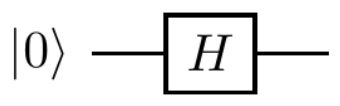
\includegraphics[width = 10em]{images/2.jpg}
\end{center}
Notice that, the outcome, $$
\Ket{0}\mapsto \frac{1}{\sqrt{2}}(\Ket{0} + \Ket{1})
$$ is truly \textbf{uniformly random}.

\subsubsection{Can we have a security analysis mechanism to verify that the bit generated is truly random?}
One fair question is, when we use such a device to generator random bit, is there a good way to verify that the random bit produced is truly random, with the manufacturer having no way to know which bit it is (or any other adversaries, as a problem that some pseudo-random generators would have)?\\

\noindent What we want here, also, is a black-box analysis, just so that anyone who uses it can verify using only inputs and outputs, without any further knowledge about the internal working of the device. \textbf{This is the question of device independence}:

\begin{definition}[\textbf{Device Independence}]
A protocol is \textbf{device independent} if its \textbf{security} doesn’t depend on \underline{trusting the devices on which it is implemented}. In other words, it has no reliance on trusting the third party who supply you with the devices.
\end{definition}

\begin{idea}
Here are few things to note:
\begin{itemize}
    \item Our process cannot be deterministic: otherwise, an all powerful adversary can always figure out a way to fool the deterministic verification process.
\end{itemize}
\end{idea}

\begin{definition}[\textbf{Randomness Expansion}]
Starting from an initial seed of \underline{private} \underline{randomness} (completely unknown to any other party), \textbf{randomness expansion} is the process of extending this to a larger amount of randomness that remains completely private.
\end{definition}

\begin{definition}[\textbf{Entropy}]\label{def:entropy}
Let $\mathbf{X} \in \{x_1, \ldots, x_k\}$ be a \textbf{discrete random variables}, then we can define the \textbf{entropy function} as $$
    H(\mathbf{X}) = -\underset{i\in [k]}{\sum}\prt{\Pr[\mathbf{X} = x_i]\log_2\Pr[\mathbf{X} = x_i]}
    $$
\end{definition}

\begin{theorem}
\hl{We will need the number of bits of $m \approx 2\cdot \lceil pn \rceil - (1-p)\log_2(1-p) - p\log_2p$ in order to randomly select and test.}
\end{theorem}
\begin{proof}
Here are the set-ups:
\begin{enumerate}[Step 1:]
    \item[Step 0:] Let Alice and Bob start with \underline{$m$-bit private key} they already agreed upon. Let them \textbf{respectively} generate \underline{$n$ qubit states}. Let there be a publicly agreed-upon \underline{$0< p < 1$}.
    \item Alice and Bob first select $\lceil pn \rceil$ of the $n$ putative states they generated as pairs to test. Since each test requires $2$ bits to test, it requires a total of $\boxed{2\cdot \lceil pn \rceil}$ bits to test the states.
    \item Recall definition \ref{def:entropy}. Well, in our case, $\mathbf{X}$ can be either 1) outputting $0$ state or 2) outputting $1$ state. So, the total \textbf{entropy} is: $$
    H(\text{output}) = -\Pr[\text{output} = 0]\log_2\Pr[\text{output} = 0]-\Pr[\text{output} = 1]\log_2\Pr[\text{output} = 1],
    $$ where we know that we have set the probability for outputting $1$ to be $p$, so $(1-p)$ for outputting $0$. So, in particular, we have $$
    H(\text{output}) = \boxed{-(1-p)\log_2(1-p)-p\log_2p}.
    $$

    Thus, to ensure selecting from at $1$ state, we need at least $$
    \boxed{m \approx 2\cdot \lceil pn \rceil - (1-p)\log_2(1-p) - p\log_2p}
    $$
\end{enumerate}
\end{proof}

\begin{remark}[Why does this help?]
If the adversary has manipulated the device that produces the pairs, then they need to be sure that they haven’t altered the pairs that Alice and Bob are testing on. But they cannot know in advance which pairs that will be, and so they cannot risk manipulating anything. \textbf{(This security requirement can formally be shown using Chernoff bound.)}
\end{remark}

\begin{remark}
In the fraction $p$ of pairs where a CHSH test is performed, we get at least 1 bit of randomness out: Alice’s measurement result is \underline{always chosen at random}. In fact, Bob’s result will be \underline{partially correlated} to Alice’s, so we should be able to extract some more randomness from this as well, but we ignore this possibility for the sake of simplicity. Thus in the end we create \hl{$(2 - p)n$ bits of randomness}.
\end{remark}

\section{Loopholes in Bell Tests}
When \textbf{hidden variables} were introduced in the beginning of this chapter, some assumptions were made to simplify expositions. These are not such big problems in physical realities and experiments. But, when it comes to cryptography, these would be the \textbf{loopholes} that the adversaries can leverage to violate Bell tests by \textbf{not satisfying one or more of these assumptions}. We define some key loopholes below:

\begin{definition}[\textbf{Detector Efficiency Loophole}]
In reality, there are likely cases where a device simply fails to detect something, \eg a photon flying by. That is why, each device should have an \textbf{efficiency parameter $\eta$} that factors in such failure probabilities by only requiring a probability of $\eta$ for the \underline{measurement to succeed}.

\noindent \textbf{Adversarial attach example:} An adversary can give a perfect detector in some cases but leverage the leeway allowed by $(1-\eta)$ failure probability to deliberately choose to \underline{fake a failure whenever their eavesdropping attempts fail}.
\end{definition}

\begin{definition}[\textbf{Locality Loophole}]
Alice and Bob should have their respective random measurement settings, observations of the measurements, observables, etc. However, if their distance, $L$, is not far enough, and since information can be transmitted up to the speed of light, $c$, then it only takes \underline{$\frac{L}{c}$} for some of the information to be exchanged between the two supposedly independent systems, potentially making them in each other's \textbf{locality}, failing the non-locality assumption. \textbf{This is called a locality loophole.}
\end{definition}

\begin{definition}[\textbf{Free-Will Loophole}]
The idea of ``free will" here is a shorthand for saying that the choices are made randomly and are not influenced by any factors that could also be influencing the measurement outcomes. Particularly, Alice and Bob needs to choose their measurement settings \underline{truly randomly}. However, due to the non-locality requirement, they only have $\frac{L}{c}$ time to make the random choice. So, in many practical cases, it is possible that they don't have such a truly-random generator that gives them respectively a truly random bit in $\frac{L}{c}$-time. One of Alice and Bob not having this capability of free-will is called the \textbf{free-Will Loophole}.
\end{definition}

\begin{remark}
The goal to close these loopholes is to make it \underline{extremely unlikely} that any hidden variables could influence both the \textbf{choice of measurement settings} and \textbf{the outcomes} \underline{simultaneously}, thus maintaining the integrity of the experiment.
\end{remark}


\end{document}